\documentclass[a4paper, 12pt]{article}

\usepackage{geometry}
\geometry{left=2cm, right=2cm, top=2cm, bottom=2cm}
\usepackage{wrapfig}
\usepackage{cmap}
\usepackage{mathtext} 
\usepackage[T2A]{fontenc}
\usepackage[utf8]{inputenc}
\usepackage[english,russian]{babel}	

\usepackage{amsfonts,amssymb,amsthm,mathtools}
\usepackage{amsmath}
\usepackage{icomma} 

\usepackage{graphicx} 
\graphicspath{{picturies/}}
\usepackage{wrapfig}

\usepackage{array,tabularx,tabulary,booktabs}
\usepackage{longtable}
\usepackage{multirow}

\usepackage{caption}
\captionsetup{labelsep=period}

\renewcommand{\phi}{\varphi}
\newcommand{\eps}{\varepsilon}
\newcommand{\parag}[1]{\paragraph*{#1:}}
\newcommand{\mysec}[1]{\begin{center}\section*{#1}\end{center}}

\author{Радькин Кирилл Б01-005}
\title{3.2.4 Свободные колебания в электрическом контуре}
\date{9.12.21}

\graphicspath{{pictures/}}

\begin{document}
    \maketitle

    \parag{Цель работы} исследование свободных колебаний в колебательном контуре
    
    \parag{В работе используются} генератор импульсов, электронное реле, магазин сопротивлений, магазин емкостей, индуктивность, электронный осциллограф, универсальный мост

    \section*{Теоретическое введение}

    \begin{wrapfigure}{l}{0.35\linewidth} 
        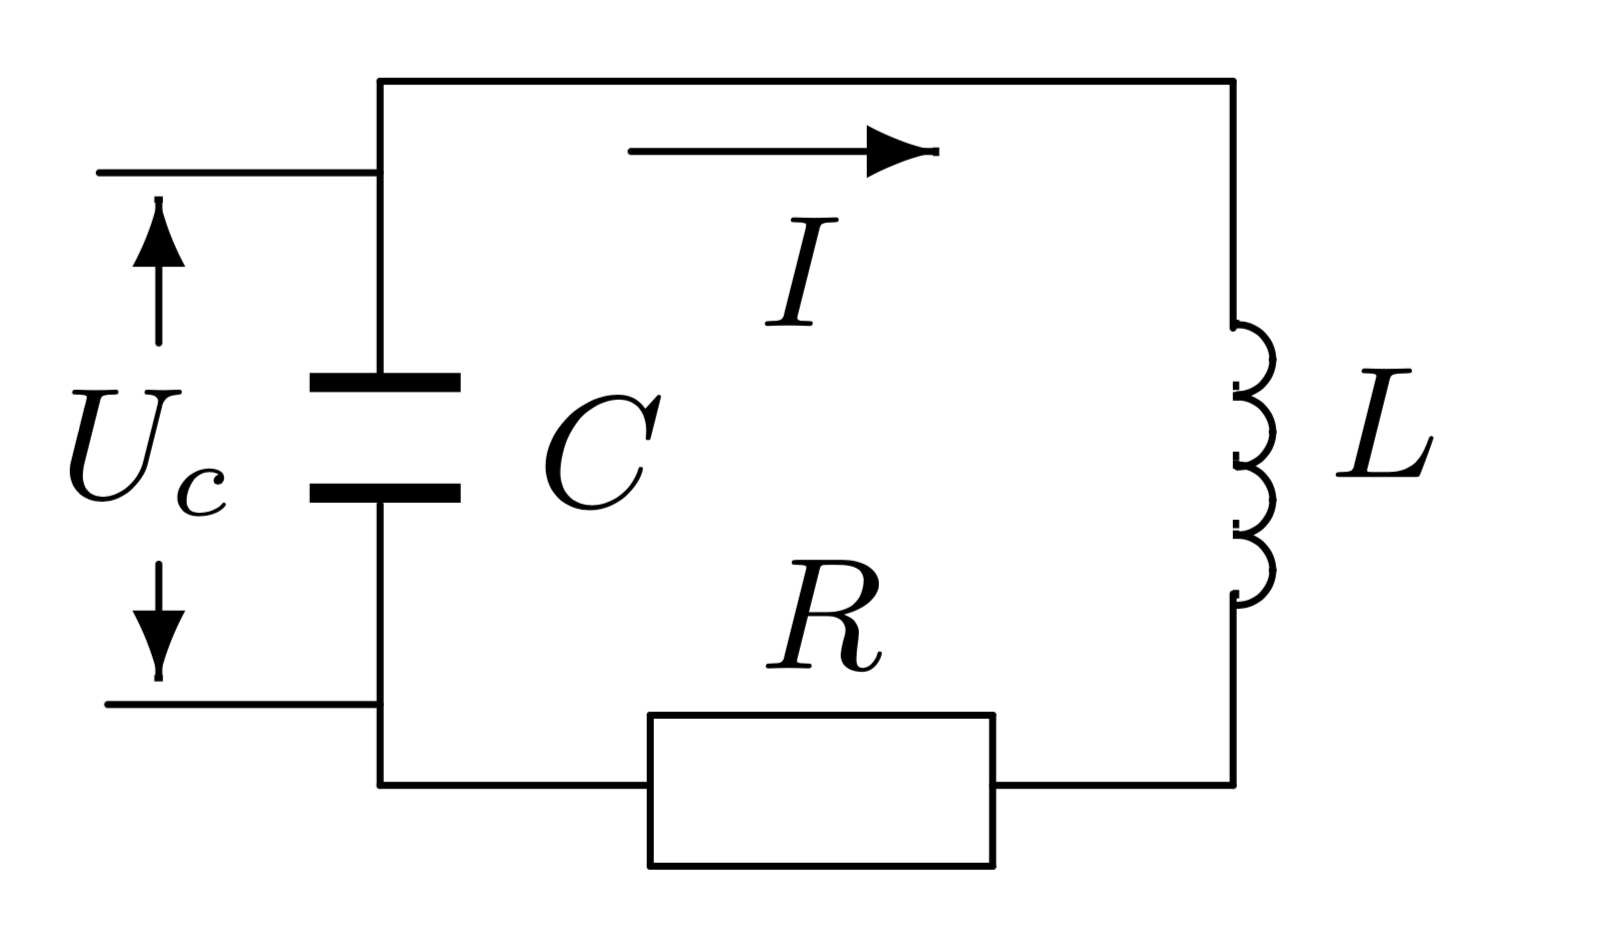
\includegraphics[width=6cm]{RLC}
        \caption{Колебательный контур}
        \label{RLC}
    \end{wrapfigure}

    Основное уравнение колебательного контура 

    \begin{equation}\label{ddot I}
    \ddot{I} + 2\gamma\dot{I} + \omega_0^2I = 0
    \end{equation}

    Где $ \gamma = \dfrac{R}{2L} $ --- коэффициент затухания, $ \omega_0^2 = \dfrac{1}{LC} $ --- собственная частота контура. Решением этого уравнения являются затухающие колебания:

    \begin{equation}\label{}
    I = A e^{-\gamma t} \cos (\omega t - \theta)
    \end{equation}

    Здесь $ \omega = \sqrt{\omega_0^2 - \gamma^2} $. Можно записать решение \eqref{ddot I} и для напряжения:

    \begin{equation}\label{}
    U_C = U_0 \dfrac{\omega_0}{\omega} e^{-\gamma t}\cos (\omega t - \theta)
    \end{equation}

    В контуре со слабым затуханием $ (\omega \backsimeq \omega_0) $ верна \textbf{формула Томпсона} для периода: 

    \begin{equation}\label{}
    T = \dfrac{2\pi}{\omega_0} \backsimeq  \dfrac{2\pi}{\omega} = 2\pi\sqrt{LC}
    \end{equation}

    Режим работы контура, при котором $ \gamma = \omega_0 $, называется \textbf{критическим}. Его сопротивление равно 

    \begin{equation}\label{}
    R_{кр} = 2\sqrt{\dfrac{L}{C}}
    \end{equation}

    Потери затухающих колебаний принято характеризовать через \textbf{добротность} и \textbf{логарифмический декремент затухания}: 

    \begin{equation}\label{Q}
    Q = 2\pi \dfrac{W}{\Delta W} = \dfrac{1}{R} \sqrt{\dfrac{L}{C}} \quad - \quad \text{Добротность, потери энергии}
    \end{equation}
    \begin{equation}\label{theta}
    \Theta = \dfrac{1}{n} \gamma T = \dfrac{1}{n} \ln \dfrac{U_k}{U_{k+n}}  \quad - \quad \text{Лог. декремент, потери амплитуды}
    \end{equation}

    \section*{Экспериментальная установка}    
    
    Исследуемый колебательный контур состоит из индуктивности $ L $,
    ёмкости $ С $ и резистора $ R $ (рис. \ref{RLC}). Конденсатор контура заряжается
    короткими одиночными импульсами, после каждого из которых в контуре
    возникают свободные затухающие колебания. Подав напряжение
    с конденсатора на осциллограф, можно по картине, возникающей на
    экране осциллографа, определить период колебаний в контуре, исследовать
    затухание колебаний и определить основные параметры колебательного
    контура.

    Картину колебаний можно представить не только в координатах ($ U, t $), но и в координатах ($ U, \dot{U} $), или, как говорят, на фазовой
    плоскости. В этих координатах кривая незатухающих колебаний ( $ \gamma = 0 $)
    имеет вид эллипса (или окружности - при одинаковых амплитудах $ U $
    и $ \dot{U} $), а картина реальных колебаний изображается сворачивающейся
    спиралью. 


    \begin{wrapfigure}{r}{0.35\linewidth} 
        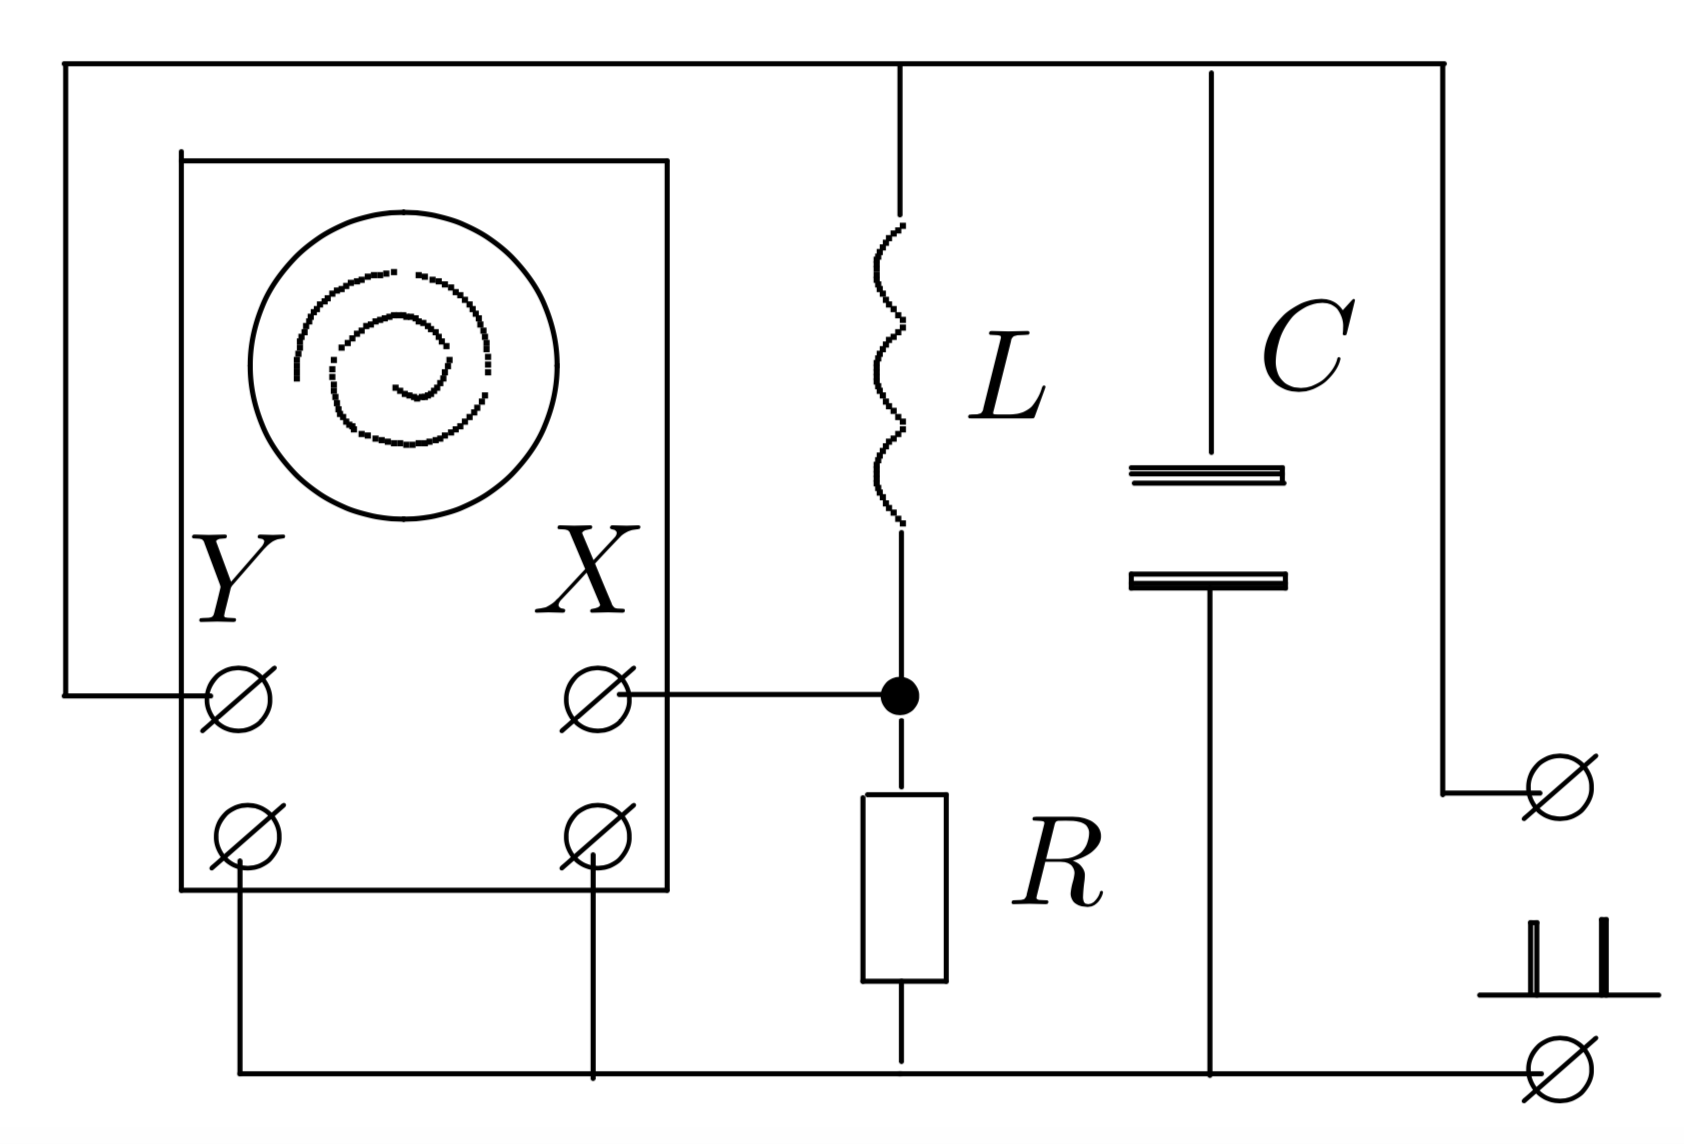
\includegraphics[width=6cm]{Fase}
        \caption{Фазовый режим}
        \label{Fase}
    \end{wrapfigure}

    Схема подключения осциллографа для изучения колебаний на фазовой плоскости представлена на рис. \ref{Fase}. На вертикальный вход осциллографа подаётся напряжение $ U_C $ с конденсатора, а на горизонтальный --- напряжение с резистора $ U_R $.

    На рис. \ref{lab} приведена схема для исследования свободных колебаний в контуре типа рис. \ref{RLC}. Колебания наблюдаются на экране осциллографа.

    Для периодического возбуждения колебаний в контуре используется
    генератор импульсов Г5-54. С выхода генератора по коаксиальному кабелю импульсы поступают на колебательный контур через электронное
    реле, смонтированное в отдельном блоке ( или на выходе генератора).
    Реле содержит диодный тиристор1 $ D $ и ограничительный резистор $ R_1 $.
    Импульсы заряжают конденсатор $ С $. После каждого импульса генератор
    отключается от колебательного контура, и в контуре возникают
    свободные затухающие колебания. Входное сопротивление осциллографа
    велико ($ \backsimeq 1$ МОм), так что его влиянием иа контур можно пренебречь.

    \begin{figure}[h]
        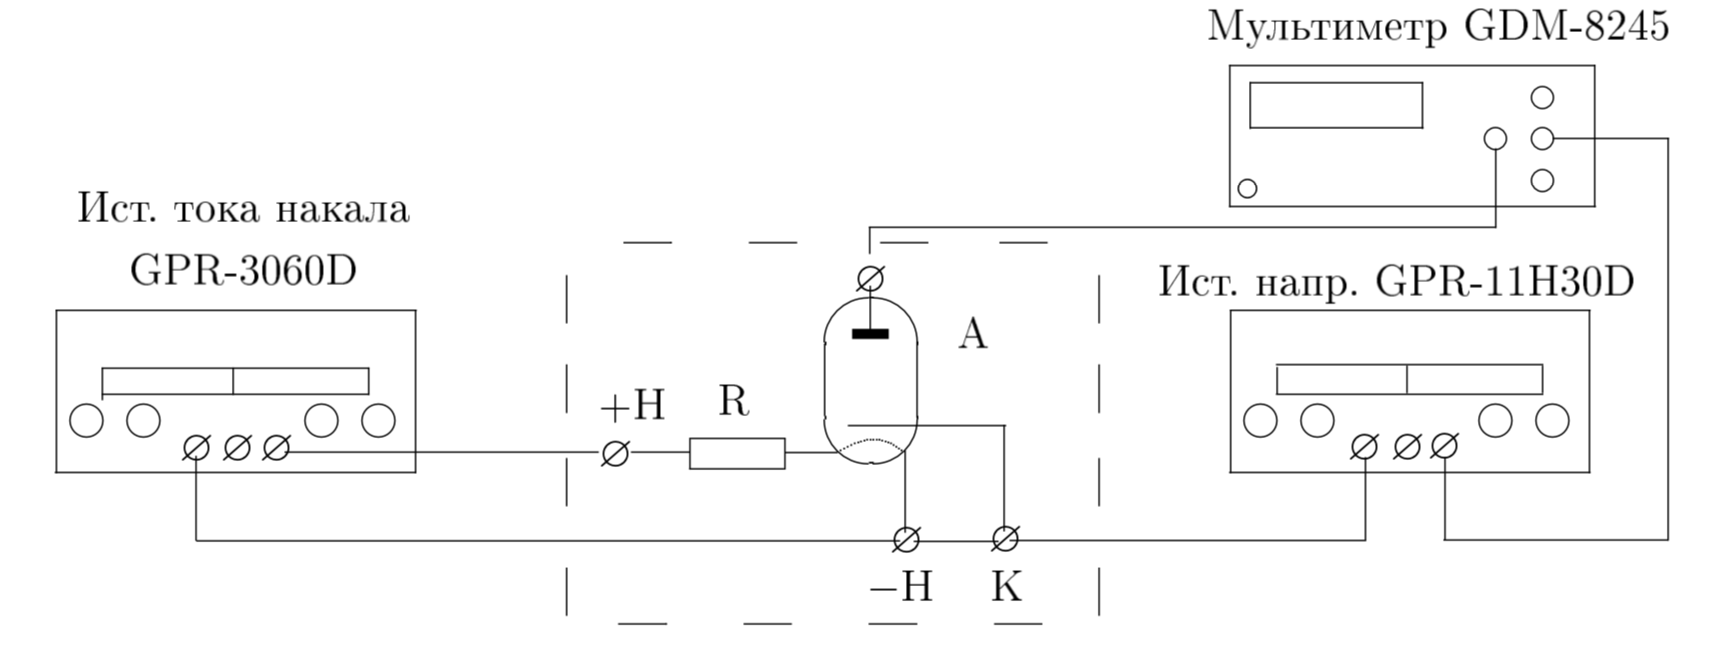
\includegraphics[width=15cm]{lab}
        \caption{Схема экспериментальной установки}
        \label{lab}
    \end{figure}

    Для получения устойчивой картины затухающих колебаний используется
    режим ждущей развёртки с синхронизацией внешними импульсами,
    поступающими с выхода "<синхроимпульсы"> генератора.

    \section*{Ход работы}

    \begin{enumerate}
        \item Настроим установку
        \item Установим на магазине сопротивлений величину $R = 0$; на магазине емкостей~---~величину $C = 0.02$ мкФ.
        \item Прокалибруем горизонтальную ось осциллографа по известному периоду повторения импульсов: для этого
        \begin{itemize}
            \item подберем частоту развёртки осциллографа, при которой расстояние $x_0$ между импульсами, поступающими с генератора занимает почти весь экран
            \item измерим на экране расстояние $x$, которое занимают несколько полных периодов $n$, рассчитаем период колебаний контура: $T = \dfrac{T_0 \cdot x}{n \cdot x_0}$
        \end{itemize}
        Изменяя емкость от $0.02$ мкФ до $0.9$ мкФ, проведем измерения периодов:
        
        \begin{tabular}{|c|c|}\hline
            $C$, мкФ & $T$, мс \\ \hline
            0.02 & 0.45 \\ \hline
            0.03 & 0.59 \\ \hline
            0.04 & 0.94 \\ \hline
            0.05 & 0.78 \\ \hline
            0.06 & 0.85 \\ \hline
            0.07 & 0.85 \\ \hline
            0.08 & 0.95 \\ \hline
            0.09 & 1.06 \\ \hline
        \end{tabular}

        \item Приняв $L = 200$ мГн, рассчитаем емкость $C$, при которой частота собственных колебаний контура будет равна $\nu_0 = 5$ кГц: $C = 5$ нФ.
        Рассчитаем также $R_{кр} = 12$~кОм.

        \item Установим на магазине емкость, близкую к рассчитаной. Увеличивая сопротивление от $0$ до $R_{кр}$, зафиксируем сопротивление, при котором колебательный режим переходит в апериодический: $R_{кр_{эксп}} = 8.8$ кОм.
        \item Установим сопротивление $R \simeq 0.1 \cdot R_{кр_{эксп}}$, получим картину затухающих колебаний (рис. \ref{zatuh_koleb}).

        Для расчета логарифмического декремента затухания $\Theta$ по формуле $\Theta = \dfrac{1}{n} \cdot \dfrac{U_k}{U_{k+n}}$, измерим амплитуды, разделенные целым числом периодов $n$.

        \begin{tabular}{|c|c|c|c|c|} \hline
            $R$, Ом & $n$ & $U_k$ & $U_{k+n}$ & $\Theta$ \\ \hline
            900 & 3 & 2 & 0.4 & 0.54\\ \hline
            1100 & 3 & 2.2 & 0.4 & 0.57\\ \hline
            1300 & 2 & 2.4 & 0.6 & 0.69\\ \hline
            1500 & 2 & 2.6 & 0.5 & 0.82\\ \hline
            1700 & 2 & 2.7 & 0.4 & 0.95\\ \hline
            1900 & 2 & 2.8 & 0.4 & 0.97\\ \hline
            2100 & 2 & 2.9 & 0.3 & 1.13\\ \hline
            2300 & 2 & 3   & 0.2 & 1.35\\ \hline
            2500 & 2 & 3   & 0.2 & 1.35\\ \hline
        \end{tabular}

        \begin{wrapfigure}{r}{0.7\linewidth}
            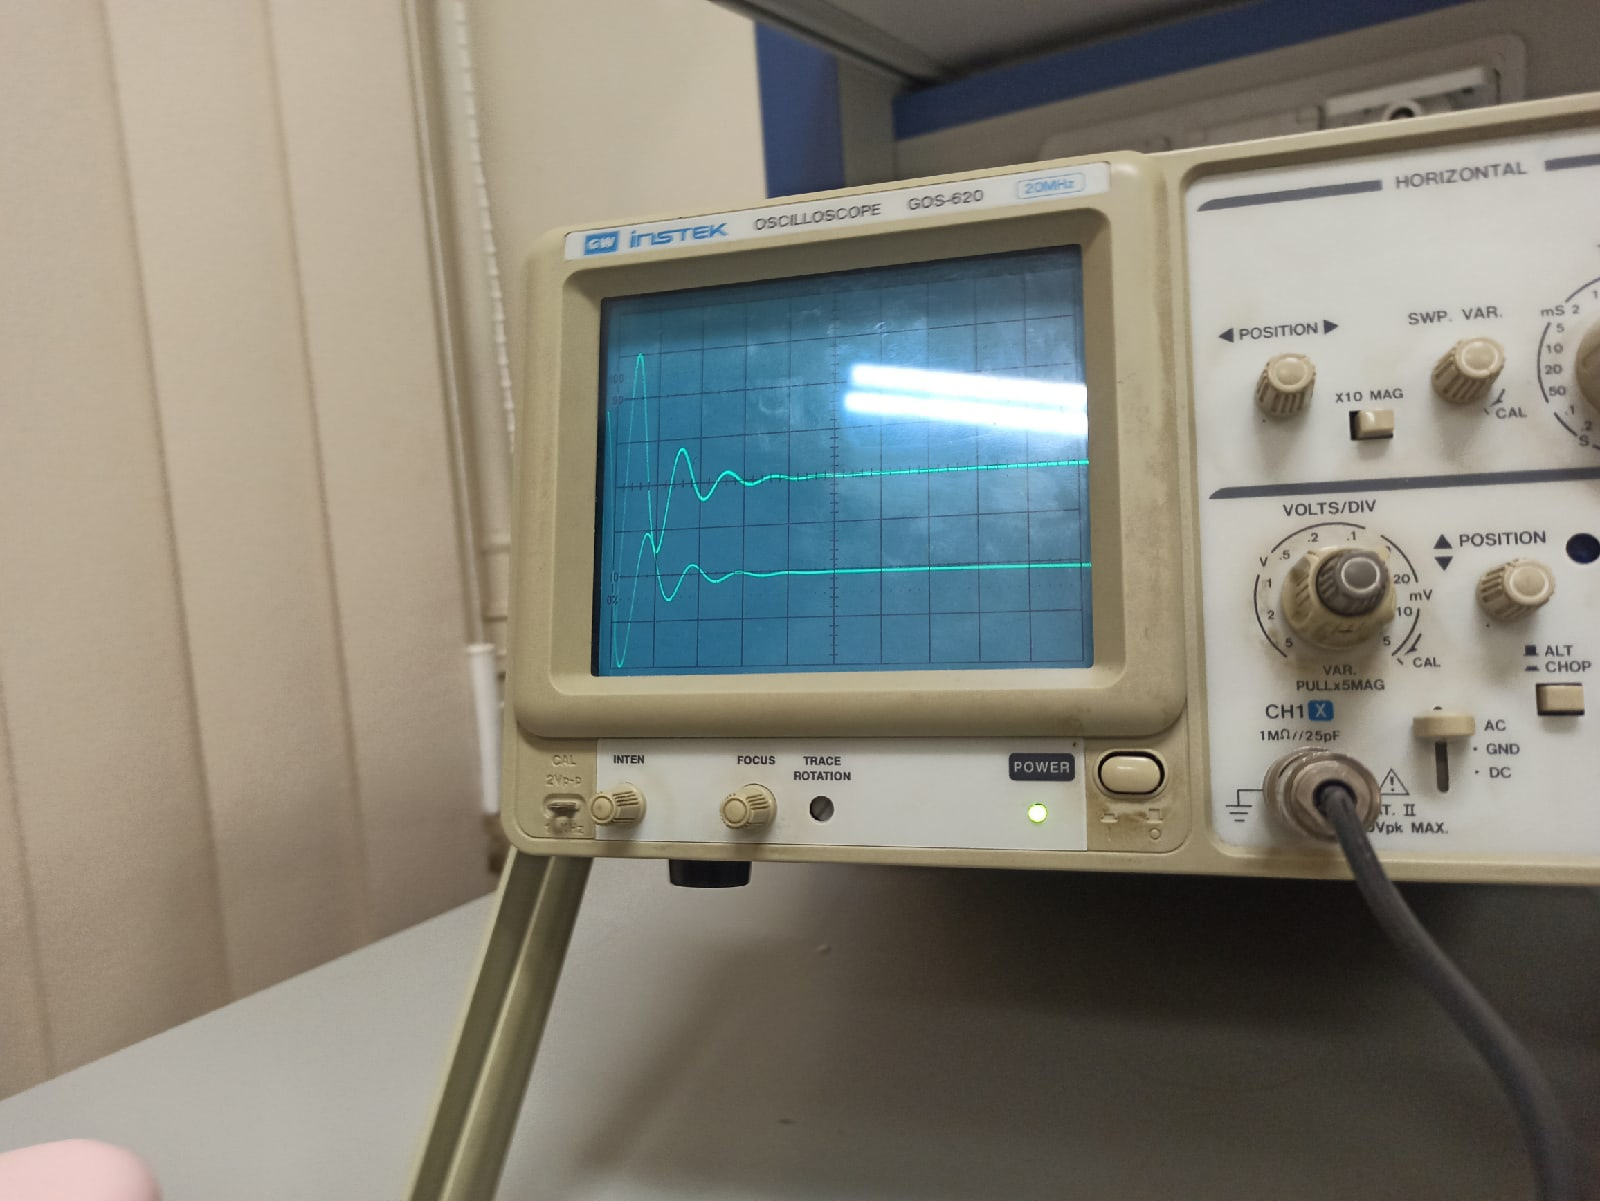
\includegraphics[scale=0.25]{zatuh_koleb.jpg}
            \caption{Затухающие колебания}
            \label{zatuh_koleb}
        \end{wrapfigure}

        \item Настроим осциллограф для наблюдения затухающих колебаний на фазовой плоскости и пронаблюдаем за изменением спирали при увеличении $R$ от $0.1 \cdot R_{кр}$ до $0.3 \cdot R_{кр}$ (одна из спиралей на рис. \ref{spiral}).
        
        \begin{wrapfigure}{r}{0.7\linewidth}
            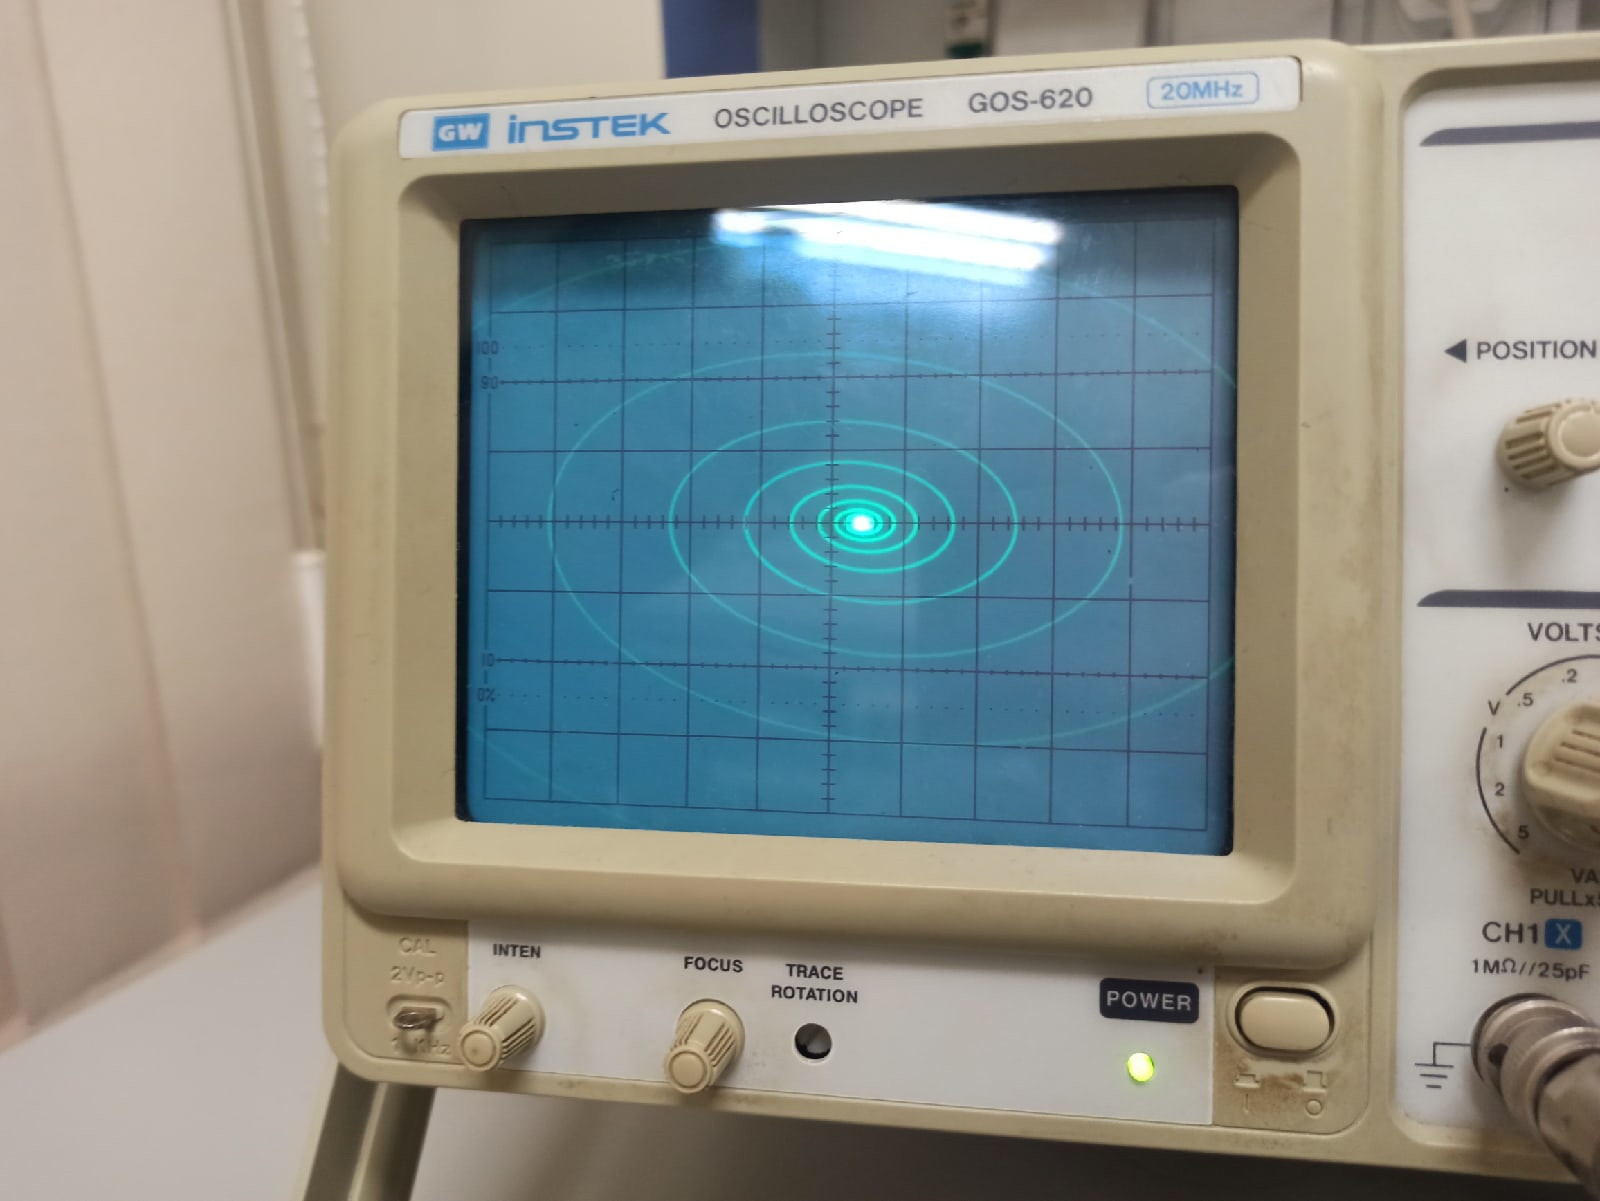
\includegraphics[scale=0.25]{spiral.jpg}
            \caption{Спираль}
            \label{spiral}
        \end{wrapfigure}

        \item Рассчитаем экспериментальные и теоретические значения периодов и построим график (рис. \ref{graph1}) $T_{эксп} = f(T_{теор})$
        
        \begin{tabular}{|c|c|} \hline
            $T_{эксп}$, мс & $T_{теор}$, мс \\ \hline
            0.45 & 0.39 \\ \hline
            0.59 & 0.49 \\ \hline
            0.95 & 0.56 \\ \hline
            0.79 & 0.63 \\ \hline
            0.85 & 0.69 \\ \hline
            0.85 & 0.74 \\ \hline
            0.96 & 0.79 \\ \hline
            1.06 & 0.84 \\ \hline
        \end{tabular}

        \begin{wrapfigure}{r}{0.5\linewidth}
            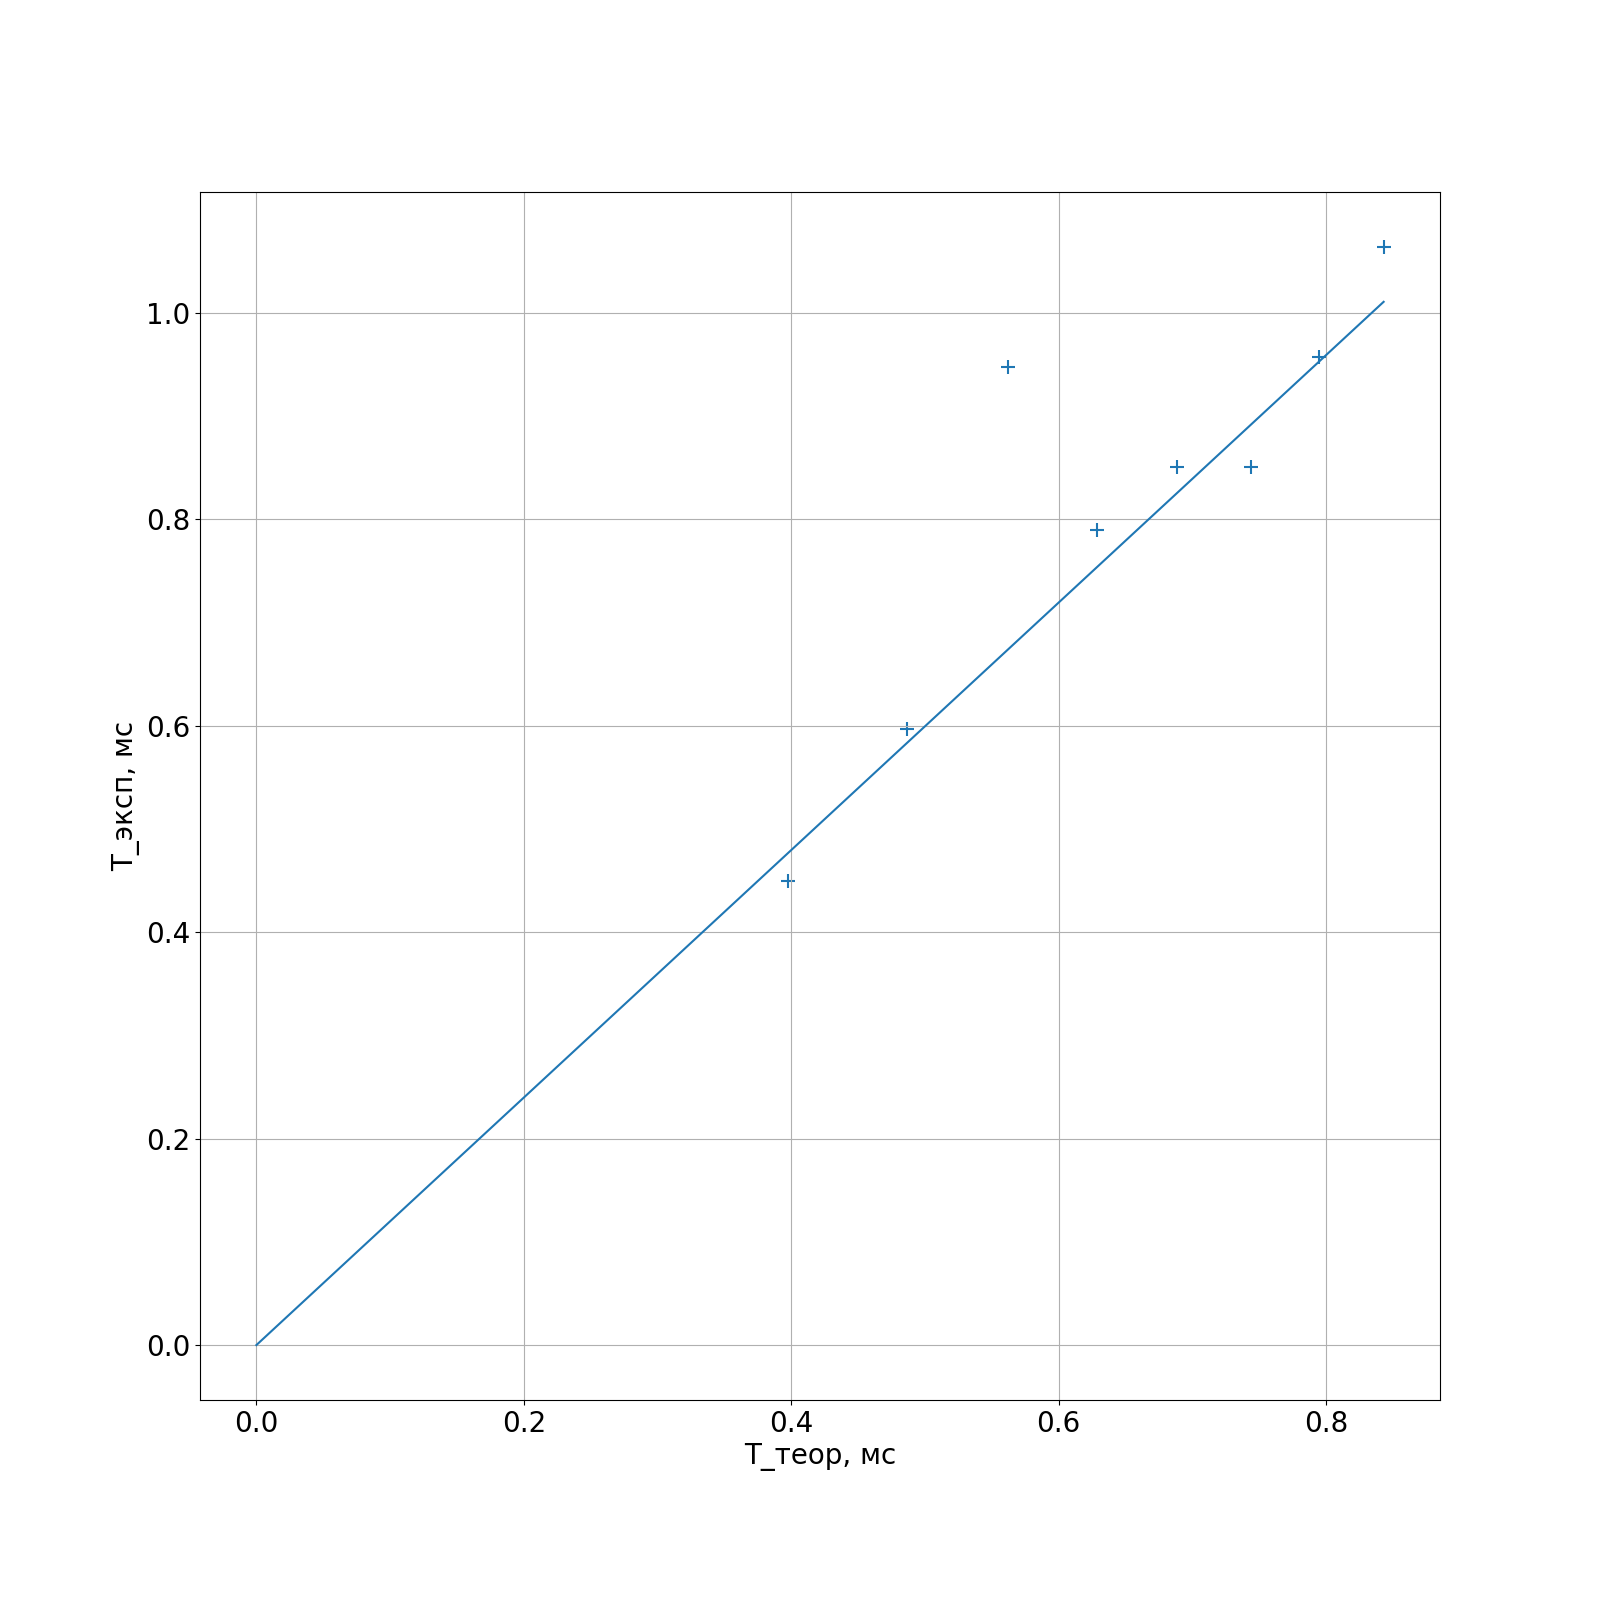
\includegraphics[scale=0.4]{graph1.png}
            \caption{$T_{эксп}$ от $T_{теор}$}
            \label{graph1}
        \end{wrapfigure}        

        \item Рассчитаем знаения $\Theta$ и $R_{конт} = R_l + R$. Построим график в координатах $\dfrac{1}{\Theta^2} = f \left( \dfrac{1}{R_{конт}^2} \right)$ (рис. \ref{graph2}).
        Определим $R_{кр}$ по наклону прямой: $R_{кр} = 11623$ Ом.

        \begin{wrapfigure}{r}{0.7\linewidth}
            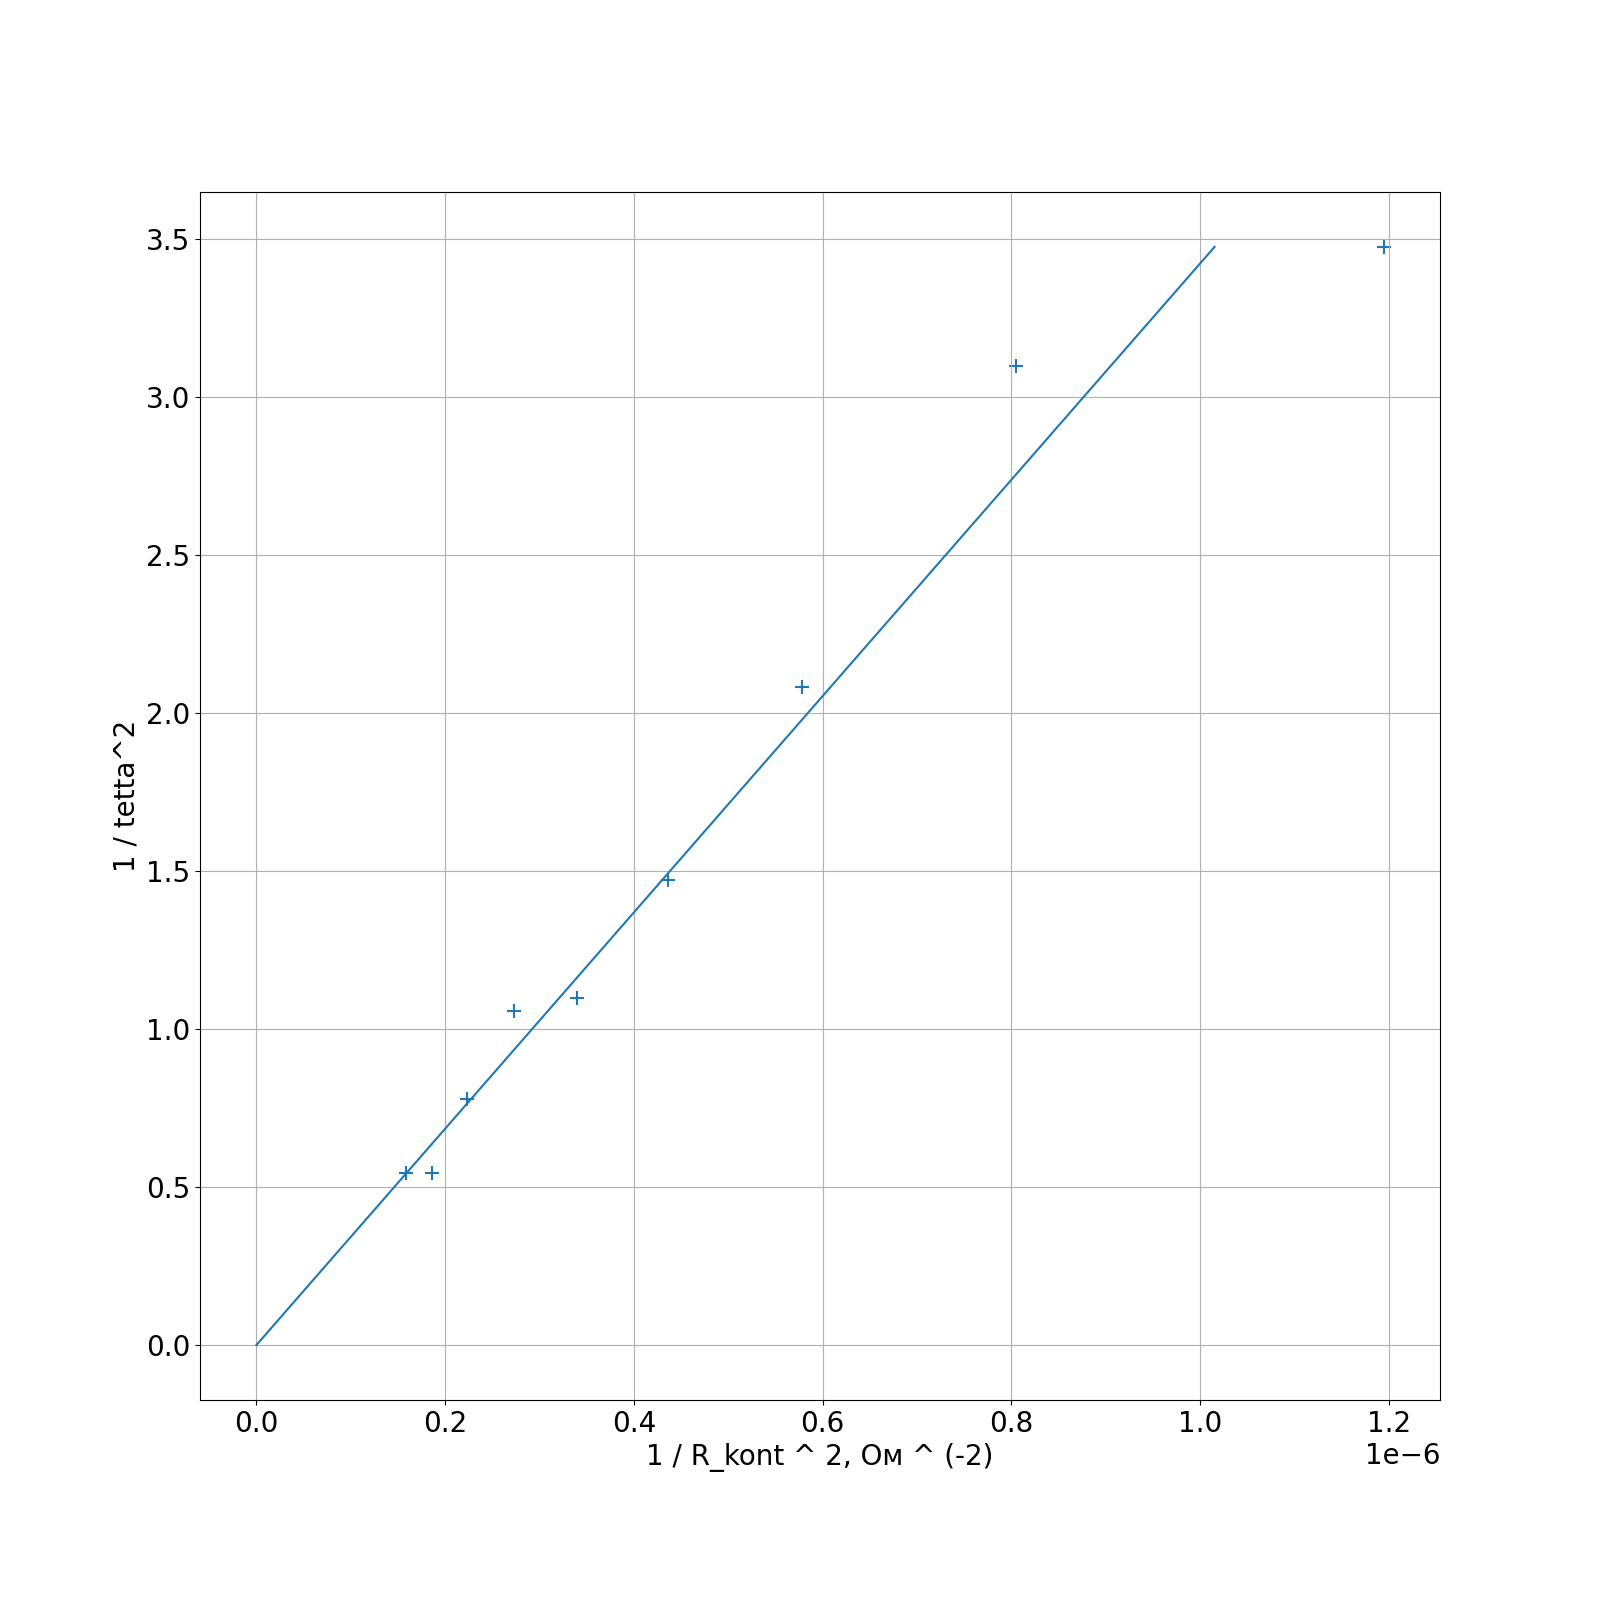
\includegraphics[scale=0.4]{graph2.png}
            \caption{$\dfrac{1}{\Theta^2} = f \left( \dfrac{1}{R_{конт}^2} \right)$}
            \label{graph2}
        \end{wrapfigure}

        \item Рассчитаем $R_{кр}$ по формуле $R_{кр} = 2 \cdot \dfrac{L}{C}$ и сравним с ранее рассчитанными значениями.\\
        $R_{кр_{теор}} = 12649$ Ом\\
        $R_{кр_{граф}} = 11623$ Ом\\
        $R_{кр_{эксп}} = 8800$  Ом

        \item Рассчитаем добротность контура для максимального и минимального значений $\Theta$ и сравним с расчетом $Q$ через параметры $R, L, C$.\\

        Через $Q = \dfrac{\pi}{\Theta}$:\\
        $Q_{max} = 5.86$, $Q_{min} = 2.32$\\

        Через $Q = \dfrac{1}{R} \cdot \sqrt{\dfrac{L}{C}}$:\\
        $Q_{max} = 6.91$, $Q_{min} = 2.51$
    \end{enumerate}
\end{document}